\documentclass[11pt]{amsart}
\usepackage{geometry}                % See geometry.pdf to learn the layout options. There are lots.
\geometry{letterpaper}                   % ... or a4paper or a5paper or ... 
%\geometry{landscape}                % Activate for for rotated page geometry
%\usepackage[parfill]{parskip}    % Activate to begin paragraphs with an empty line rather than an indent
\usepackage{graphicx}
\usepackage{amssymb}
\usepackage{epstopdf}
\usepackage[english]{babel}
\usepackage{graphicx}
\DeclareGraphicsRule{.tif}{png}{.png}{`convert #1 `dirname #1`/`basename #1 .tif`.png}

\title{Visualizing Build Diversity through Dimensionality Reduction}
\author{Conor Dowling and Alex Brigham}
%\date{}                                           % Activate to display a given date or no date

\begin{document}
\maketitle


\section{Introduction}

The goal of this project was to provide a tool to visualize the changes caused by the massive AP item changes. Specifically, we wanted to create a tool that would allow users to see changes in build diversity both across champions and within champions. Because there are so many different AP items and champions available to choose from, it is impractical to try to display all of that raw data in a single page. This lead us to use dimensionality reduction to allow users to compare all champions at once or many builds simultaneously. In addition to the two dimensions of the graph, we use time as a third dimension in order to visualize differences between champion builds across patches, regions, or tiers in solo queue.\\

\section{Data Pipeline}
\subsection{RiotWatcher}
The first step in the data pipeline is collecting the match data for the matches provided for the challenge. We used a Python module called RiotWatcher (github.com/pseudonym117/Riot-Watcher) to interface with the Riot API and systematically request the data for each game.\\

\subsection{MongoDB}
We chose to store the match data in a MongoDB database, creating a table for each set of matches provided. MongoDB seemed like an obvious choice because it was easy to setup and could store the match data in raw JSON format with no editing required.\\

\subsection{MapReduce}
Once we had gathered all of the data, we used MongoDB's built-in map-reduce functionality to extract the data that we wanted from each game and aggregate that data within regions and patches. We performed three separate map-reduce operations to obtains statistics on how many times champions were played, which items they built, and which builds were most popular.\\

\subsection{Sci-Kit Learn}
We used the Python library SciKit Learn to perform our dimensionality reduction. We tested out a couple of the different decomposition algorithms provided including PCA (Principle Component Analysis), LDA (Linear Discriminant Analysis) and Gaussian Random Projection.\\


\section{Visualization}
To create the visualizations, we used D3.js, also known as the Data Driven Documents Javascript library. We based the original version on an example on the D3 examples page (http://bl.ocks.org/WilliamQLiu/bd12f73d0b79d70bfbae), but heavily modified it to add in addition functionality such as tooltips and hover-to-zoom functionality. One of our old designs connected to a MongoDB database to run queries on the data provided, but the response time was too long, so we ran the required queries and cached the data in files on the web server.\\


\section{Data Sets}
\subsection{Build Diversity Across Champions}

For this data set, we looked at the frequency at which champions purchased specifically finished AP items. We included items that provided any ability power but excluded items which were used as part of recipes such as Amplifying Tome or Needlessly Large Rod. We took the frequency to be the total number of times a champion purchased an item divided by the total number of games that champion was played.\\ 

We created vectors of these frequencies for each champion, region, and tier combination, including data points for aggregates of all tiers and regions. Next, we filtered out champions that averaged less than one AP item built per game across all of their vectors. This prevents our dimensionality reduction from focusing too much on whether a champion built AP items and more towards which ones they chose to build.\\

Taking these vectors of 32 AP items, we used a Gaussian Random Projection to map these vectors two a two-dimensional plane. A Gaussian Random Projection is a method of dimensionality reduction which tries to preserve distances between points as it projects a dataset into a lower dimension, in this case, two.\\

This type of analysis is interesting because not only does it allow you to view a high-dimensional space easily, but it will also pick out some trends in the data. Simply graphing all of the points generated, we see a group in the lower right and three or four branches extending out from it. Upon closer examination, there is a branch for for champions that tend to build Rod of Ages such as Singed, Kassadin, Swain, and Ryze, and another for support champions that might build Frost Queen's Claim or Banner of Command which includes Bard, Nami, and Sona.\\

\begin{figure}[h!]
  \caption{All points plotted in two dimensions.}
  \centering
    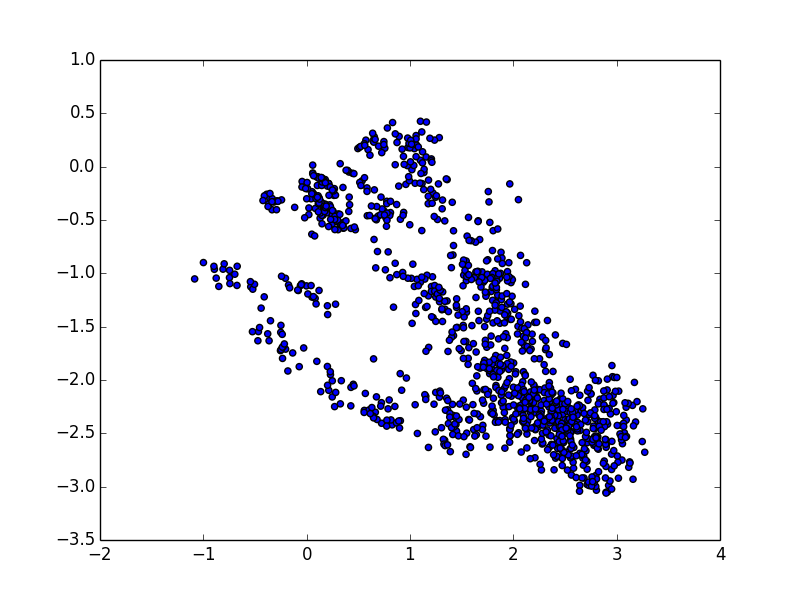
\includegraphics[width=0.8\textwidth]{figure_1.png}
\end{figure}

You might wonder how well these two dimensions are able to illustrate the difference in builds. While there are no metrics provided by the SciKit Learn implementation of Gaussian Random Projection, we were able to get some metrics using a PCA (Principle Component Analysis) which was able to explain roughly 50 percent of the total variance, 36 percent across one axis and 14 across the other. Comparing these two methods, we concluded that the Gaussian Random Projection was better suited for our analysis because we cared more about the distance between each pair of points.\\

\subsection{Build Diversity Within Champions}

To examine diversity within champions, we took a slightly different approach. Instead of looking strictly at item frequencies, we took build order into account. We looked at the first three major items and which boots a player purchased in a given game. If the player was not able to purchase all of these items, the game was not counted. In this case, we considered all major items because it allowed us to look at AP tanks and extended the tool to all champions instead of just AP champs.\\

Each data point was a vector of all of the items with all values initialized to zero. We assigned the first item completed a value of four, the second item three, the third two, and the boots one. Then to compare two builds, the distance between them was just the distance between their vectors. For instance, if two builds were the same except for their boots, the distance would be two. If two builds had their first and second items switched, the distances would also be two, and if two builds shared no items in common, their distance would be 20.\\

We took the 100 most popular builds for each champion, region, tier combination and performed the same Gaussian Random Projection.\\


\subsection{Champion Build Order Statistics}

To accompany our visualization of builds within each champion, we also generated statistics for the most popular items for each champions. Instead of overall frequency of purchase we instead looked which items different champions chose to buy first, second, or third. For instance, we see that Annie builds Rod of Ages as her first item 40 percent of the time and as her second item only 9 percent of the time.\\

\section{Future Work}

One aspect of our project that could use some improvement is the statistical analysis. Currently, small sample sizes can create outliers in the data and could give the user the wrong impression. Although the graph is already pretty involved, some notion of confidence intervals could be helpful to show the user how much the data should be trusted.\\


\section{Conclusions}

Using our tool, it was fairly easy to find trends in the data. One of the most useful features shows how much a champion moved in our 2D plane between the current and the last dataset. By simply switching between patches, we could easily see that Evelynn, Elise, Ezreal, Ekko, and Kayle were among the most changed by the changes. Granted, factors such as changes to the actual champions, as in Elise's case, confound the effects of the AP item changes on their builds, but we can see the influence that the addition of the Runeglaive enchantment had on the builds of these champions. While the Runeglave changes were the most obvious, by looking at individual champions, we can see the rise of Rylai's in popularity among champions such as Karthus.\\

Overall, I think it provides an interesting interface through which to view trends in champion builds and investigate the effects of changing a variable such as patch, region, or tier, to see how it affected different groups of players.\\



\end{document}  